%%%%%%%%%%%%%%%%%%%%%%% file template.tex %%%%%%%%%%%%%%%%%%%%%%%%%
%
% This is a general template file for the LaTeX package SVJour3
% for Springer journals.          Springer Heidelberg 2010/09/16
%
% Copy it to a new file with a new name and use it as the basis
% for your article. Delete % signs as needed.
%
% This template includes a few options for different layouts and
% content for various journals. Please consult a previous issue of
% your journal as needed.
%
%%%%%%%%%%%%%%%%%%%%%%%%%%%%%%%%%%%%%%%%%%%%%%%%%%%%%%%%%%%%%%%%%%%
%
% First comes an example EPS file -- just ignore it and
% proceed on the \documentclass line
% your LaTeX will extract the file if required
\begin{filecontents*}{example.eps}
%!PS-Adobe-3.0 EPSF-3.0
%%BoundingBox: 19 19 221 221
%%CreationDate: Mon Sep 29 1997
%%Creator: programmed by hand (JK)
%%EndComments
gsave
newpath
  20 20 moveto
  20 220 lineto
  220 220 lineto
  220 20 lineto
closepath
2 setlinewidth
gsave
  .4 setgray fill
grestore
stroke
grestorew
\end{filecontents*}
%
\RequirePackage{fix-cm}
%
%\documentclass{svjour3}                     % onecolumn (standard format)
%\documentclass[smallcondensed]{svjour3}     % onecolumn (ditto)
\documentclass[smallextended]{svjour3}       % onecolumn (second format)
%\documentclass[twocolumn]{svjour3}          % twocolumn
%
\smartqed  % flush right qed marks, e.g. at end of proof
%
\usepackage{graphicx}
%
% \usepackage{mathptmx}      % use Times fonts if available on your TeX system
%
% insert here the call for the packages your document requires
%\usepackage{latexsym}
% etc.
%
% please place your own definitions here and don't use \def but
% \newcommand{}{}
%
% Insert the name of "your journal" with
% \journalname{myjournal}
%
\begin{document}

\title{Citation Analysis of Computer Science%\thanks{Grants or other notes
%about the article that should go on the front page should be
%placed here. General acknowledgments should be placed at the end of the article.}
}
\subtitle{Relationship With Other Fields}

%\titlerunning{Short form of title}        % if too long for running head

\author{Sitaram Devarakonda  \and
	Dmitriy Korobskiy \and
        Tandy Warnow \and
        George Chacko }

%\authorrunning{Short form of author list} % if too long for running head

\institute{Sitaram Devarakonda,  \at
              Netelabs, NET ESolutions Corporation, McLean, VA \\
              %Tel.: +123-45-678910\\
              %Fax: +123-45-678910\\
              \email{sitaram@nete.com}           %  \\
%             \emph{Present address:} of F. Author  %  if needed
           \and
              Dmitriy Korobskiy \at
              Netelabs, NET ESolutions Corporation, McLean, VA  \\
              \email{dk@nete.com}
           \and
           Tandy Warnow \at
              Dept of Computer Science, University of Iliinois Urbana-Champaign, Champaign IL \\
              \email{warnow@illinois.edu}
           \and
           George Chacko \at
              Netelabs, NET ESolutions Corporation, McLean, VA \\
              \email{netelabs@nete.com}
}

\date{Received: date / Accepted: date}
% The correct dates will be entered by the editor

\maketitle

\begin{abstract}
Computer science as a field has experienced dramatic growth and diversification over the last twenty years. Towards an improved understanding of the structure of the field, we analyze a cohort of the computer science literature using a historiographic approach. For further insight on the features of this cohort and the flow of information within its components, we construct article level clusters whose elements are linked by citations or co-citations, and reconcile them with subject categories in the All Science Journal Classification (Scopus). [abstract is feeble and needs to be rewritten]

\keywords{Bibliometrics \and Clustering \and Research Evaluation \and Computer Science}
% \PACS{PACS code1 \and PACS code2 \and more}
\subclass{01A85 \and 01A90} %\and more}

\end{abstract}

\section{Introduction}
\label{intro}

Computer science, and its applications, has experienced rapid growth and diversification over the last twenty years. The collective influence of the Internet of Things (IoT), `big' data, accessible cloud computing, and advances in artificial intelligence have further been postulated as a recent driver for its growth and evolution~\cite{siebel2019_digital}. As also noted in a 2017 US National Academies Report~\cite{nas_2017}, ``A wide range of jobs in virtually all sectors demand computing skills to an unprecedented extent. And every academic discipline finds itself incorporating computing into its research and educational mission".

Given this powerful influence of computer science in research, some understanding its present state, structure, and relationship to other fields that goes beyond satisfying mere interest seems warranted since it would inform planning and policy making at multiple levels from national level funding all the way down to faculty hiring strategy. In using the term inform, we are mindful of (i) Greenhalgh (ii) Sarewitz and Pielke. \emph{I think that I want to cite these two without really knowing how. Greenhalgh for the limitations of positivism. Sarewitz for the limitations of allowing science to do whatever it wants to. I'd also like to see some text about (i) limited funding resources (ii) efficient use of existing resources (iiii) informing policy at multiple levels -- all directed at justifying our study. I'm not sure where to put it though. CS can also be an excellent model system for studying interdisciplinarity cite Porter and colleagues in a study on measuring interdisciplinarity~\cite{porter_measuring_2007 } observe that 'The discrepancies between disciplinary roots and research realities loom large', a reference to the challenges associated with knowledge diffusing across researchers who tend to be focused in their own areas. This concern may be especially relevant for computer science given the ubiquity of computing today and limited public funding for research. Maybe squeeze in Tandy's NAS report on interdisciplinarity. I should ping Ohid Yaqub about this too- science policy is his area.}

In a historical study of the computer science literature (419 computer articles published in 1974,  and 3,812 references cited in these articles), Salton and Bergmark made the key point that the scientific literature serves a rich source of information to study the structure and historical development of a field~\cite{salton_citation_1979}. They described the global structure of computer science as consisting of three main subareas (i) theoretical foundations, e.g., theory of computation (ii) hardware and computer systems, e.g., architecture (iii) software, e.g, programming systems.  Related areas acknowledged were  (a) mathematics of computing, e.g., numerical analysis (b) special software topics, e.g., operating systems (c) data management and database systems (d) methodologies valid for multiple applications, e.g., algebraic manipulation (e) computer applications, e.g., computer graphics (f) nontechnical aspects, e.g., computer education. 

Much in the way of growth and evolution of computing has occurred since 1974. Progressing beyond the historical triad of theoretical foundations; hardware and computer systems; and software, the Computing Classification System (CCS)~\cite{acm_ref} published by the Association for Computing Machinery now consists of 13 top-level areas that reflect a more current view of the field. This classification does address relationships with other fields under Applied Computing. However, an easy way to map scientific publications, especially interdisciplinary articles or those from adjacent fields, to the CCS classification does not exist. 

Other classification systems are available such as the All Science Journal Classification (ASJC) developed and maintained by Scopus. the Web of Science research and categorical classifications, the NSF classification system~\cite{nsf_classification}. All three rely on applying one or more journal-derived labels to articles. Disciplinary assignments using journal based classifications have been extensively discussed and critiqued~\cite{wang_large-scale_2016} [need comprehensive list of citations] with Shu and colleagues recently noting from a comparative study of the Chinese Science Citation Database (CSCD) and the Web of Science that 46\% of articles did not belong to the discipline of the journal they were published in~\cite{shu_comparing_2019}. Accordingly, article classification systems have also been developed~\cite{traag_louvain_2019,boyack_classification_2014,waltman_new_2012}, which escape some of the criticisms of journal-based classification.

In extending the work of Salton and Bergmark to the 21st century, we sought to combine journal and article based classifications in a scalable manner. Accordingly, we used a whole text search method to match records from two major data sources. (i) the dblp bibliography- a reference bibliography for computer science~\cite{dblp_ref}. We assumed that a record in dblp qualifies for a computer science label (ii) the journal based Scopus bibliography, which more comprehensively covers the physical sciences, life sciences, social sciences, and health sciences and enables easy identification of publications linked by citations. 

Using both direct citations and co-citations as the basis for clustering, we used articles from from journals and conference proceedings for the period 1996-2015. We reconciled these clusters with the the All Science Journal Classification (ASJC) developed and maintained by Scopus as well as to the CCS classification through a combination of automated and manual procedures. We describe high-level interactions of computer science within the Physical Sciences as well as with the Social Sciences, and Life Sciences. 

\section{Materials and Methods}

\emph{Data} A stable release of the dblp computer science bibliography~\cite{dblp_ref} consisting of 7,079,994 records was downloaded as dblp-2018-08-01.xml.gz. Publications were parsed from the xml source file and loaded into a PostgreSQL database. We have previously parsed, the Scopus dataset of over 72,000,000 publications into a custom schema as part of a larger data platform for research evaluation~\cite{GithubERNIE2019}. Records in the dblp dataset, were matched to Scopus identifiers using PostgreSQL's full text search feature applied to document titles. The process involves parsing all Scopus document titles into tokens, reducing the tokens into lexemes and returning vectors, which lists these lexemes. The vectors are then matched with corresponding text search vectors extracted from DBLP document titles. A rank is returned based on the frequency of matching lexemes. Only records in dblp with DOIs (4,291,130) were considered and only matches with a rank of $>$ 0.99 were accepted. This procedure resulted in a dataset of 634,100 publications with Scopus identifiers. Cited references for these were extracted from Scopus, resulting in a total of 3,960,503 nodes (publications and references) and 11,992,387 edges that represent citations of these references and publications within the dataset. This dataset is referred to as \emph{comp}.\par

\emph{Clustering by Direct Citation} Graclus is a spectral graph clustering package that computes normalized cut and ratio association for a given undirected graph~\cite{graclus_2007}. We downloaded v1.2 from the authors' website at `cs.utexas.edu'. The \emph{comp} dataset was used as input to Graclus, formatted as an undirected graph and stored in a file with a header line indicating the number of nodes and edges. Graclus requires, as a parameter, the number of clusters to be formed and we varied this parameter between 10 and 50 clusters. Using Graclus to generate 20 clusters, resulted in a set with the largest cluster containing roughly 10 times the number of nodes in the smallest one~\cite{traag_louvain_2019}. [@sitaram please add the number of nodes in the Graclus 20 clusters]. 

\emph{Clustering by Co-Citation} To build clusters using co-citations, we used variable level clustering, an approach developed by Small and Sweeney (1985)~\cite{small_clustering_1985}, with minor modifications. Variable level clustering involves applying a threshold below which all edges are dissolved then iteratively selecting edges with the highest normalized co-citation value and extracting connected components from the graph as clusters for each edge in turn. Three parameters are needed (i) a threshold or starting level based on a quantile of normalized co-citation frequency (ii) a level increment (iii) a maximum cluster size. An issue is the generation of very large clusters by chaining through low edge weights.  Thus, at each iteration, any cluster exceeding the maximum cluster size is put back into the process and a higher threshold applied. 

In our implementation of variable level clustering, we first calculated the number of citations accumulated across Scopus for all 634,100 articles in \emph{comp}. After discarding those publications without any citations, we restricted further analysis to those in the 90th percentile of citations or higher resulting in a dataset of size 50,869. We then identified 897,407 publications in Scopus that cite the 50,869 previously selected papers from \emph{comp}. The cited references in these papers were restricted to those in the set of 50,869 highly cited papers previously identified. For each of the 897,407 citing publications in turn, all possible reference pairs were generated ${n \choose x}$ where $n$ is the number of references in a publication and $x=2$. The frequency of these co-cited pairs was then computed across the dataset  and normalized using Salton's cosine formula~\cite{salton_citation_1979}. A total of 2,208,135 unique co-cited pairs were thus obtained. These data were represented in a graph where each node was a publication and the weighted edge between the pair was the normalized co-citation frequency. \par

\begin{figure}[ht]
% Use the relevant command to insert your figure file.
% For example, with the graphicx package use
  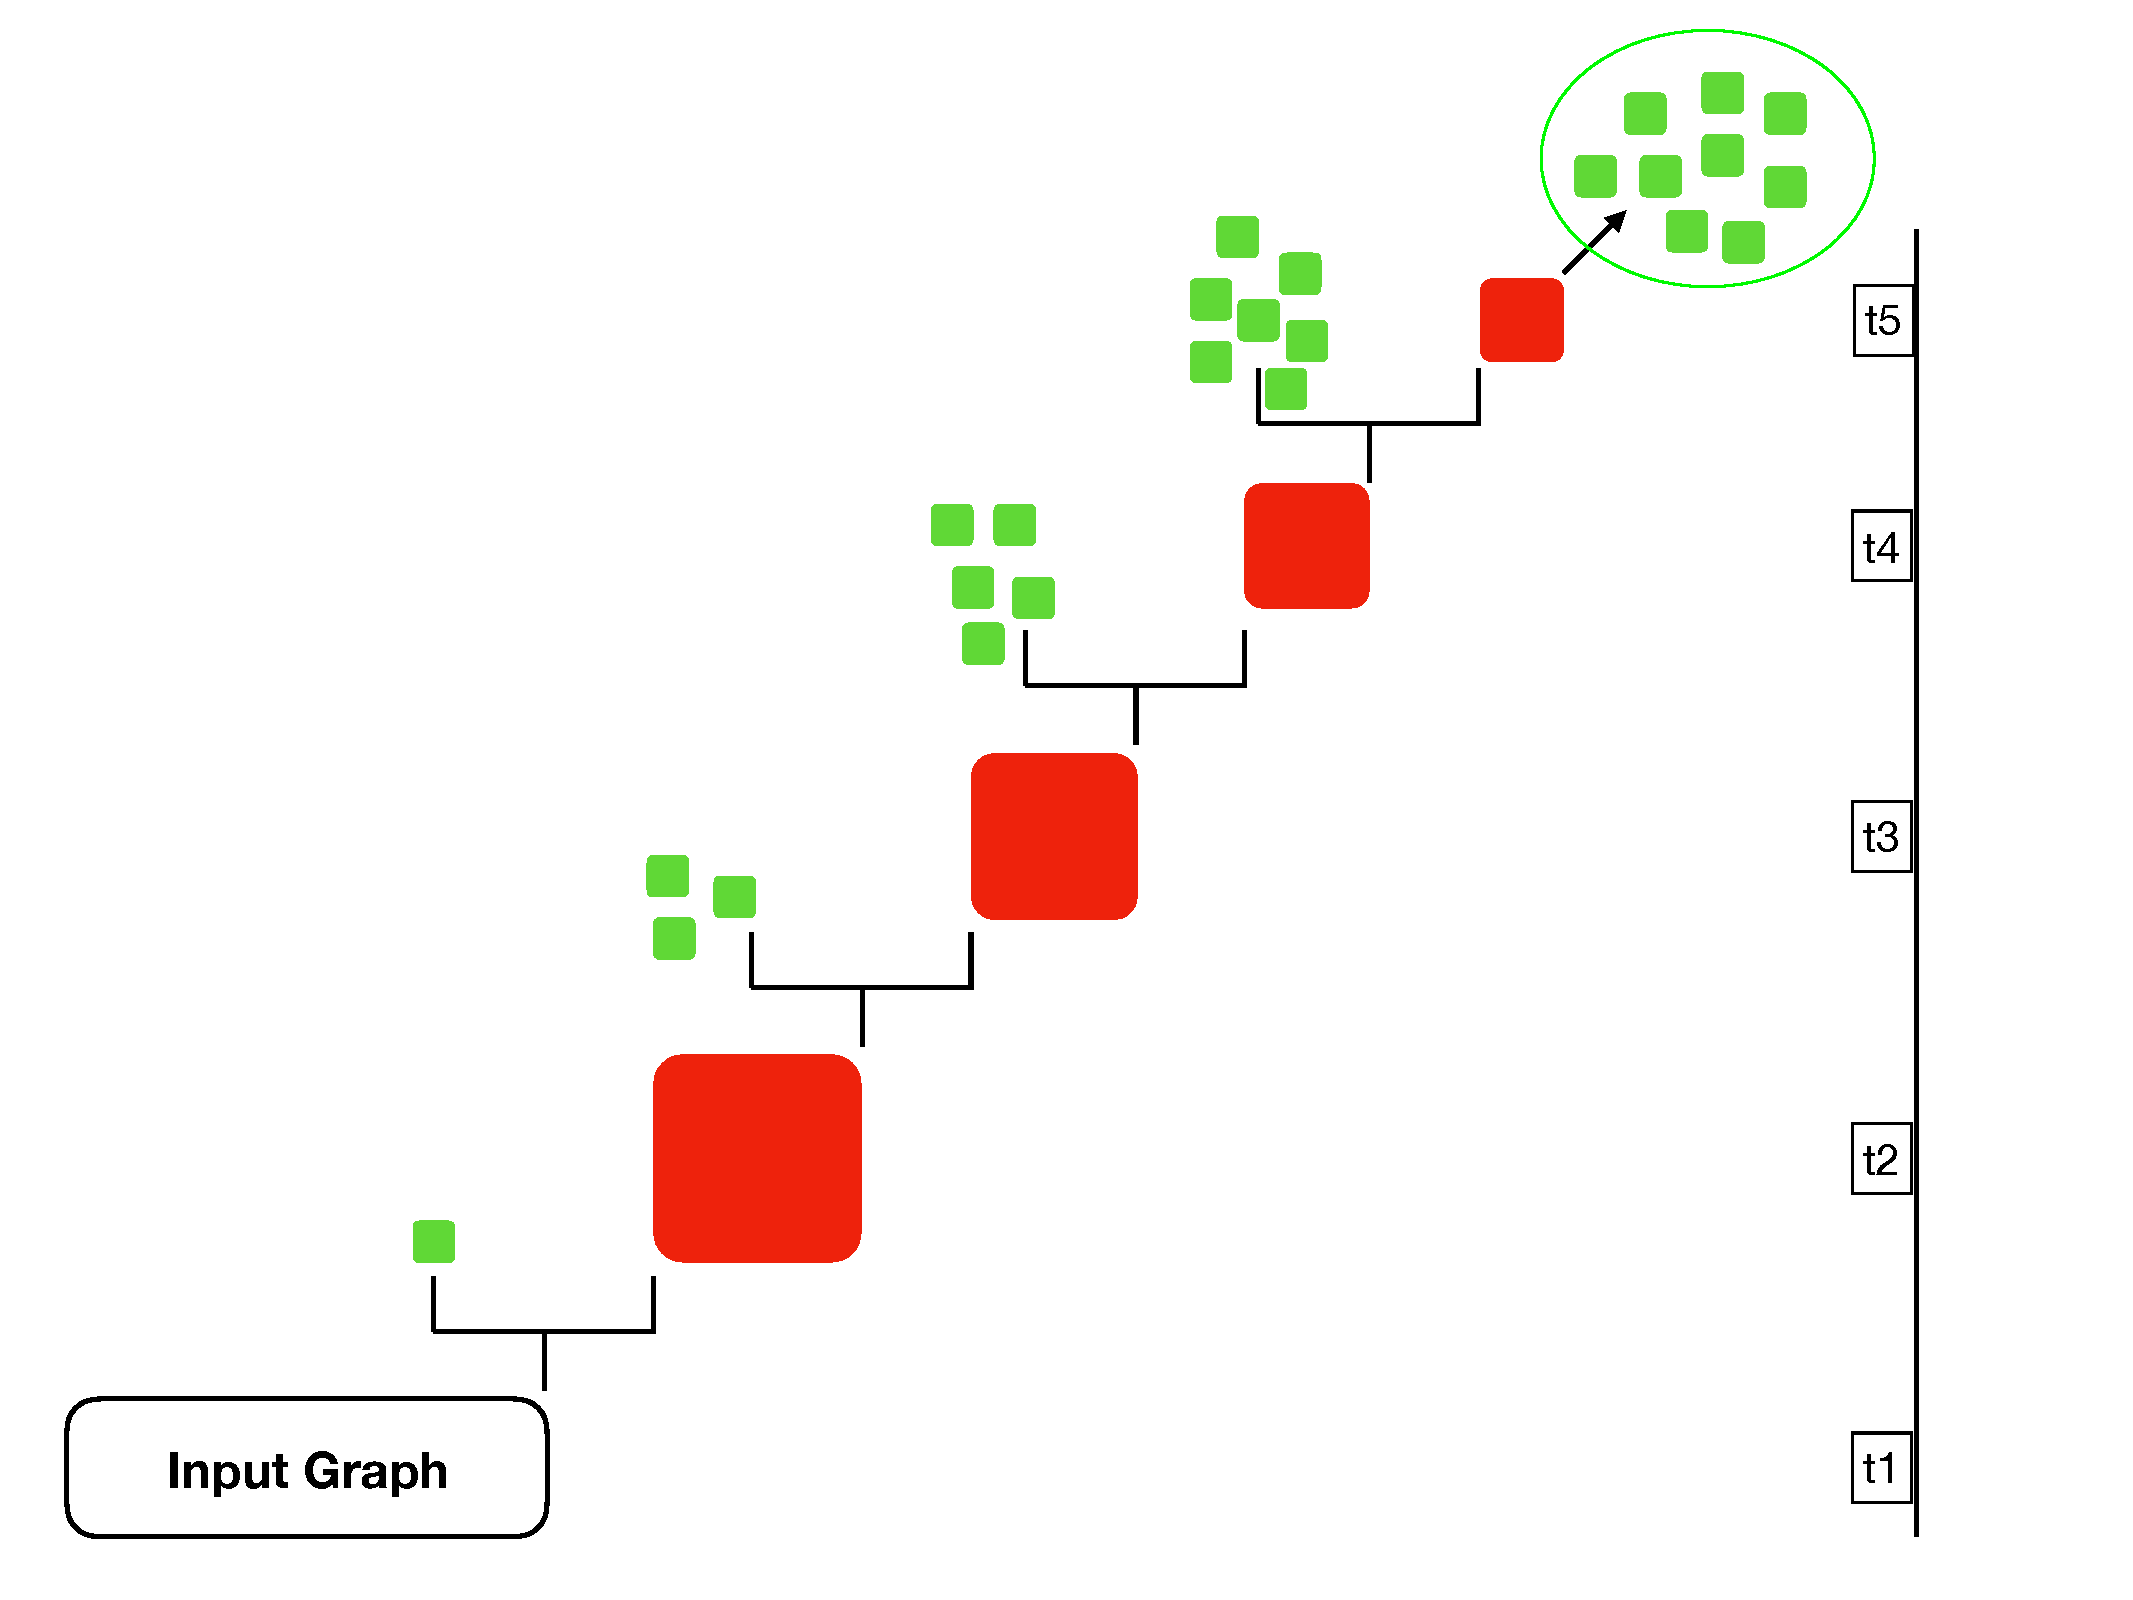
\includegraphics[scale=0.2]{vlc.pdf}
% figure caption is below the figure
\caption{Schematic representation of variable clustering protocol modified from Small and Sweeney (1985). Three parameters are specified (i) a threshold or starting level based on a quantile of normalized co-citation frequency (ii) a level increment (iii) a maximum cluster size. Input data is a set of co-cited publications with edge-weight defined by normalized co-citation frequencies. Green clusters are within the max cluster size. At the initial threshold, $t1$, a single cluster below the maximum cluster size, $mcs$ (green), along with one large cluster above it (red) are generated. As the threshold is incremented to $t2$, additional clusters of acceptable size is generated. The cascade continues to completion, which is defined by all clusters being of size less than or equal to the $mcs$. In this schematic, five rounds are adequate for the process to run to completion.}
\label{vlc_process}       % Give a unique label
\end{figure}

We applied variable clustering with initial parameters of threshold ($t$) = 0.5 (median normalized co-citation frequency), increment $i = 0.1$, and maximum cluster size, $mcs = 100$. Thus, at start, all edges below the median normalized co-citation frequency are dissolved. Clusters were formed by assembling connected components from each co-cited pair beginning with the heaviest edge weight. Clusters below size 100 were retained and any cluster larger than 200 nodes was carried over to the next round. The threshold, $t$, was then incremented by 0.1 and the process repeated while progressively incrementing $t$.  We used a bi-phasic approach where in which $t$ ranged from 0.5-0.9, after which $i$ was reduced to 0.01 for the range $0.9 <= t <= 0.99$. A final threshold of $t$=0.999 was applied to break the single remaining large cluster. All clusters generated thus, contained  less than 100 nodes.  Using this approach, 6,822 clusters containing 35,485 nodes were generated. Clusters containing only 2 nodes were then discarded bringing the total number of clusters down to 3,851. Pairwise clustering was then performed on these clusters to generate super-clusters. After 9 rounds of pairwise clustering, 13 clusters were generated resulting from agglomeration of 3,851 clusters 

\emph{need to cite Granovetter somewhere for definition of strong and weak ties that Small refers to}

\label{sec:1}
Text with citations \cite{RefB} and \cite{RefJ}.

\section{Results}
\label{sec:2}

Cite Alan Porter on expanding universe versus myopic focus. Cite Traag, Waltman, Lariviere papers. Peter Sjögårde and Per Ahlgren, Loet Leydesdorff, Caroline S. Wagner and Lutz Bornmann, Discontinuities in citation relations among journals: self-organized criticality as a model of scientific revolutions and change, Scientometrics, 10.1007/s11192-018-2734-6, 116, 1, (623-644), (2018). Antonio Perianes-Rodriguez and Javier Ruiz-Castillo, A comparison of the Web of Science and publication-level classification systems of science, Journal of Informetrics, 10.1016/j.joi.2016.10.007, 11, 1, (32-45), (2017). Qi Wang and Ludo Waltman, Large-scale analysis of the accuracy of the journal classification systems of Web of Science and Scopus, Journal of Informetrics, 10.1016/j.joi.2016.02.003, 10, 2, (347-364), (2016). Henry Small, Kevin W. Boyack and Richard Klavans, Identifying emerging topics in science and technology, 
Crossref
Overall strategy:

\begin{figure}[ht]
% Use the relevant command to insert your figure file.
% For example, with the graphicx package use
  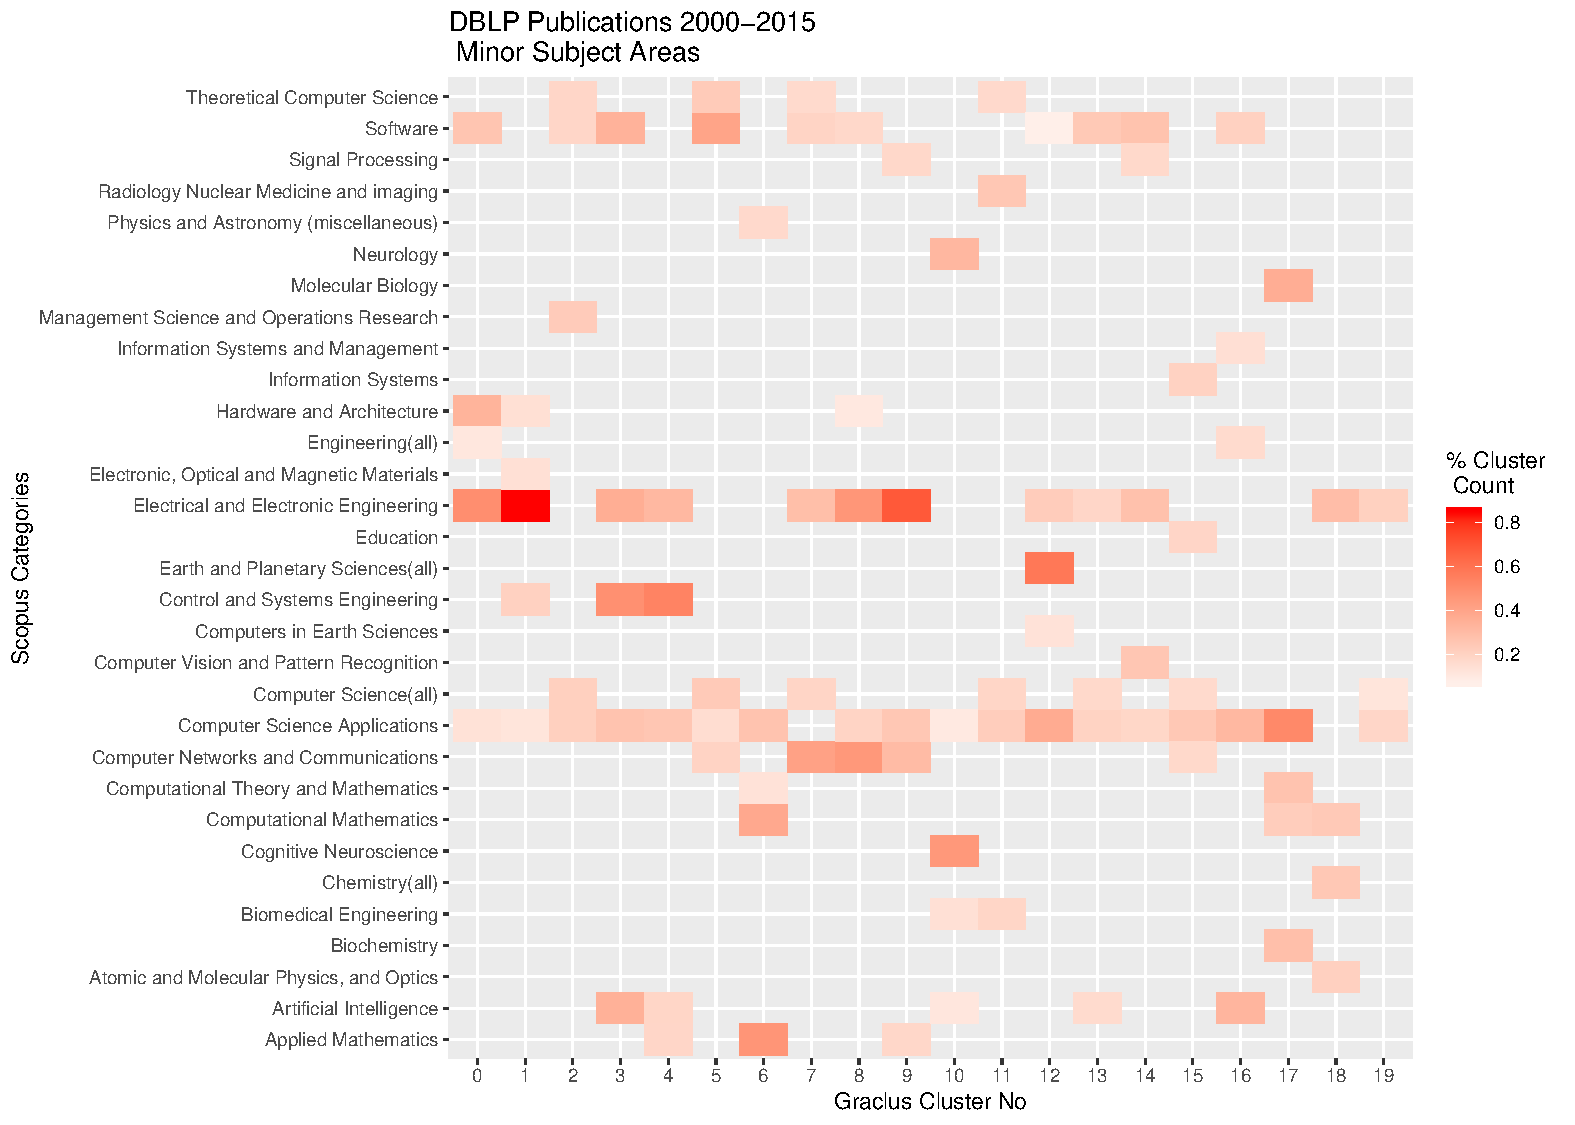
\includegraphics[scale=0.5]{scopus_dblp_graclus2.pdf}
% figure caption is below the figure
\caption{insert caption}
\label{heatmap}       % Give a unique label
\end{figure}

\begin{itemize}
\item Spectral clustering
\begin{enumerate}
\item Subset Scopus by COMP
\item Match COMP to dblp at high stringency -> reduced number of scps
 \item Harvest cited references  from Scopus
 \item Cluster articles by direct citation using Graclus to a number that meets simple optimality criteria and does not impose cognitive challenges
 \item Reconcile cluster contents to journal classification for the purpose of referencing
 \item Infer inter-cluster relationships using direct citations, co-citations, and bibliographic coupling
\end{enumerate}
\item Co-citation based clustering
\begin{enumerate}
\item Stratify by year after subsetting by COMP and restricting to article and cp only
\item Apply fractional citation counting and identify highly-cited papers
\item Calculate normalized co-citations
\item Cluster by variable clustering method of Small
\item Evaluate major co-cited pairs
\end{enumerate}
\end{itemize}


Text with citations \cite{RefB} and \cite{RefJ}.

\subsection{Subsection title}
\label{sec:2}
as required. Don't forget to give each section
and subsection a unique label (see Sect.~\ref{sec:1}).
\paragraph{Paragraph headings} Use paragraph headings as needed.
\begin{equation}
a^2+b^2=c^2
\end{equation}

% For one-column wide figures use
\begin{figure}
% Use the relevant command to insert your figure file.
% For example, with the graphicx package use
  \includegraphics{example.eps}
% figure caption is below the figure
\caption{Please write your figure caption here}
\label{fig:1}       % Give a unique label
\end{figure}
%
% For two-column wide figures use
\begin{figure*}
% Use the relevant command to insert your figure file.
% For example, with the graphicx package use
  \includegraphics[width=0.75\textwidth]{example.eps}
% figure caption is below the figure
\caption{Please write your figure caption here}
\label{fig:2}       % Give a unique label
\end{figure*}
%
% For tables use
\begin{table}
% table caption is above the table
\caption{Please write your table caption here}
\label{tab:1}       % Give a unique label
% For LaTeX tables use
\begin{tabular}{lll}
\hline\noalign{\smallskip}
first & second & third  \\
\noalign{\smallskip}\hline\noalign{\smallskip}
number & number & number \\
number & number & number \\
\noalign{\smallskip}\hline
\end{tabular}
\end{table}


%\begin{acknowledgements}
%If you'd like to thank anyone, place your comments here
%and remove the percent signs.
%\end{acknowledgements}


% Authors must disclose all relationships or interests that 
% could have direct or potential influence or impart bias on 
% the work: 
%
% \section*{Conflict of interest}
%
% The authors declare that they have no conflict of interest.


% BibTeX users please use one of
%\bibliographystyle{spbasic}      % basic style, author-year citations
\bibliographystyle{spmpsci}      % mathematics and physical sciences
%\bibliographystyle{spphys}       % APS-like style for physics
\bibliography{comp}   % name your BibTeX data base

% Non-BibTeX users please use
\begin{thebibliography}{}
%
% and use \bibitem to create references. Consult the Instructions
% for authors for reference list style.
%
\bibitem{RefJ}
% Format for Journal Reference
Author, Article title, Journal, Volume, page numbers (year)
% Format for books
\bibitem{RefB}
Author, Book title, page numbers. Publisher, place (year)
% etc
\end{thebibliography}

\end{document}
% end of file template.tex

